
\section{Methodology and tools used}

\subsection{Android studio with kotlin}
To develop our application, we decided to use Android Studio and Kotlin because they offer many advantages in Android development. Indeed, Kotlin is an efficient programming language for building Android applications. 
Kotlin has a concise syntax and interesting features, like intelligent casts and extension functions that reduces the amount of code to write.
Kotlin also offers support for functional programming concepts such as lambda functions and extension functions. It grants us the right to write clean and modular code easily. Kotlin is also well supported by Android Studio, the Integrated Development Environment (IDE) we have used to develop our application.\newline

Android Studio was our choice of IDE. It gives us an great programming tool, while allowing us to emulate easily smartphones to test on those devices the interfaces and functionalities of our application. \newline

In order to structure our project, we created various activities for each part of our project. It is divided into three parts. First of all, we created an activity for the user to describe their needs. For that, we created a User Interface (UI), named “general settings”. For instance, in this UI, they can tell whether they are sensitive to noise, light or crows. We will therefore decide an itinerary that is adapted to their needs. Then, we created a second activity that allows the user to choose the points of departure, arrival, but also at which time they want to leave, and the transportation mode that they want to use. All this information is used in the main activity that gives the best itinerary to the user regarding all their personal needs. \newline


\subsection{Databases and API}
In order to generate the map, we used the API OpenStreetMap (OSM). It is a collaborative mapping project that provides a free, editable map of the world. In our project, we used OSM data within Kotlin and Android Studio to generate a map of Toulouse and calculate routes between two points. By integrating OSM's API into our application, we have been able to access detailed geographical information, including roads, landmarks, and points of interest, allowing us to generate an interactive map interface within our app. Thanks to OSM, we also implemented the route calculation functionality, enabling users to input their desired start and end points and receive optimal route suggestions based on real-time OSM data. This integration allowed us to have a first itinerary without considering the user’s needs and the public transportation. \newline

Since we want to use public transportation for our application, we needed another tool than OSM to generate our routes.This is why we also integrated the Tisséo API for generating routes with public transportation in Toulouse. This API gave us access to all the data of the Tisséo transportation network, including all the buses, metros and tramways. We also had access to the public transportation timetable. This integration enabled us to generate a route at a certain time, using a combination of walking and public transportation in the city of Toulouse. By combining OSM's detailed geographical data with Tisséo's public transportation information, our application offered users a comprehensive and efficient navigation solution tailored to the unique transportation infrastructure of Toulouse. \newline

\subsection{Agile methodology and project organization}

For the organization of the project, we used Github Project.
One of the great advantages of this tool is its direct integration with the code.

First, we defined the use cases in Github Issues.
This allowed us to define the functionalities of our project and break them down into smaller tasks.
It is a perfect integration of the agile method, which allows the project to be broken down and assigned to team members.

\begin{figure}[h]
    \centering
    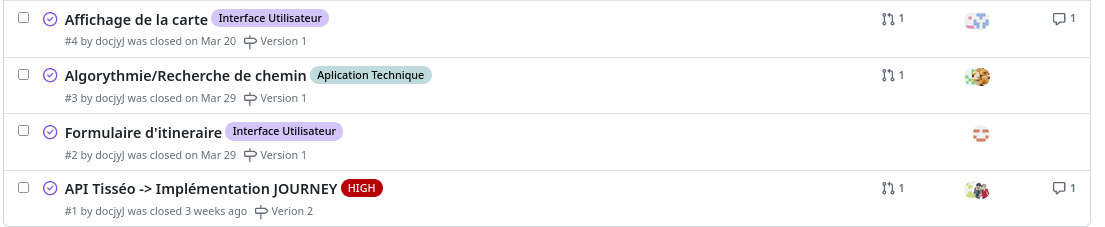
\includegraphics[width=0.8\textwidth]{img/GitHubUseCase}
    \caption{Example use case on GitHub Issue}
    \label{fig:GitHubUseCase}
\end{figure}

Then we had to bring together the different parts of the project.
Once again, Github Project allowed us to integrate this step as best as possible.
Via a pull request, we had a discussion space directly on the code.
For example in figure \ref{fig:GitHubPullRequest}, we can discuss an implementation.
These discussions allow the code to be properly integrated.

\begin{figure}[h]
    \centering
    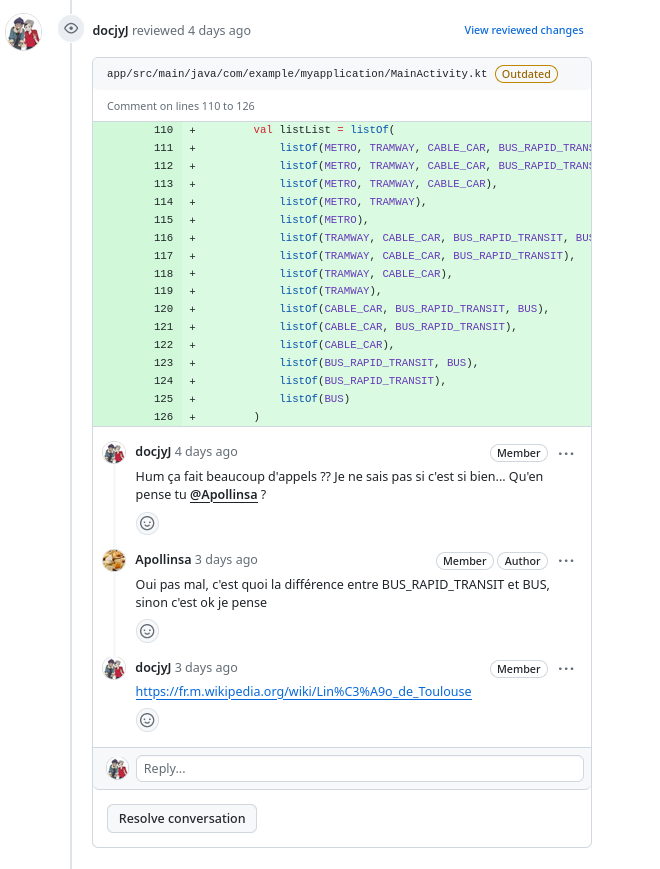
\includegraphics[width=0.4\textwidth]{img/GitHubDiscuss}
    \caption{Example of a discussion in a Pull Request on GitHub}
    \label{fig:GitHubPullRequest}
\end{figure}

\newpage

Then, Github Project allowed us to track the various unforeseen bugs.
Each person is free to add an issue, and we add it to the current sprint or for later depending on its criticality.
Even if adding tasks during the sprint is not recommended, it allowed us to adapt to the project for urgent situations.

\begin{figure}[h]
    \centering
    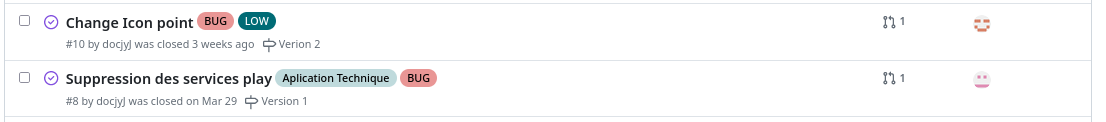
\includegraphics[width=0.8\textwidth]{img/GitHubBug}
    \caption{Example of bug reported on GitHub}
    \label{fig:GitHubBug}
\end{figure}

These three elements allow perfect integration of the agile method into our project.
In addition, GitHub project also provides several views that allow you to monitor the progress of the project.
All of these views are configurable based on the assigned sprint, labels, people, etc.
Formatting, Kanban in figure \ref{fig:GitHubKanban}, Gantt in figure \ref{fig:GitHubGant} or table,
are available to monitor the progress of the project.


\begin{figure}[h]
    \centering
    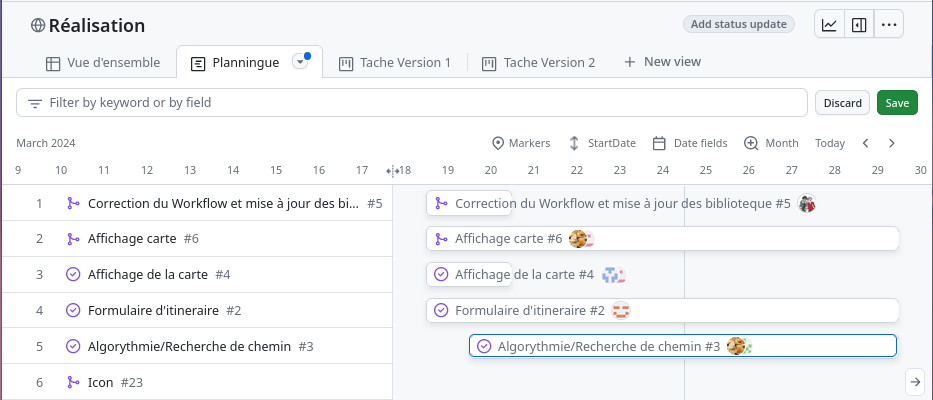
\includegraphics[width=0.8\textwidth]{img/GitHubGant}
    \caption{GitHub Project Gantt view}
    \label{fig:GitHubGant}
\end{figure}

\begin{figure}[h]
    \centering
    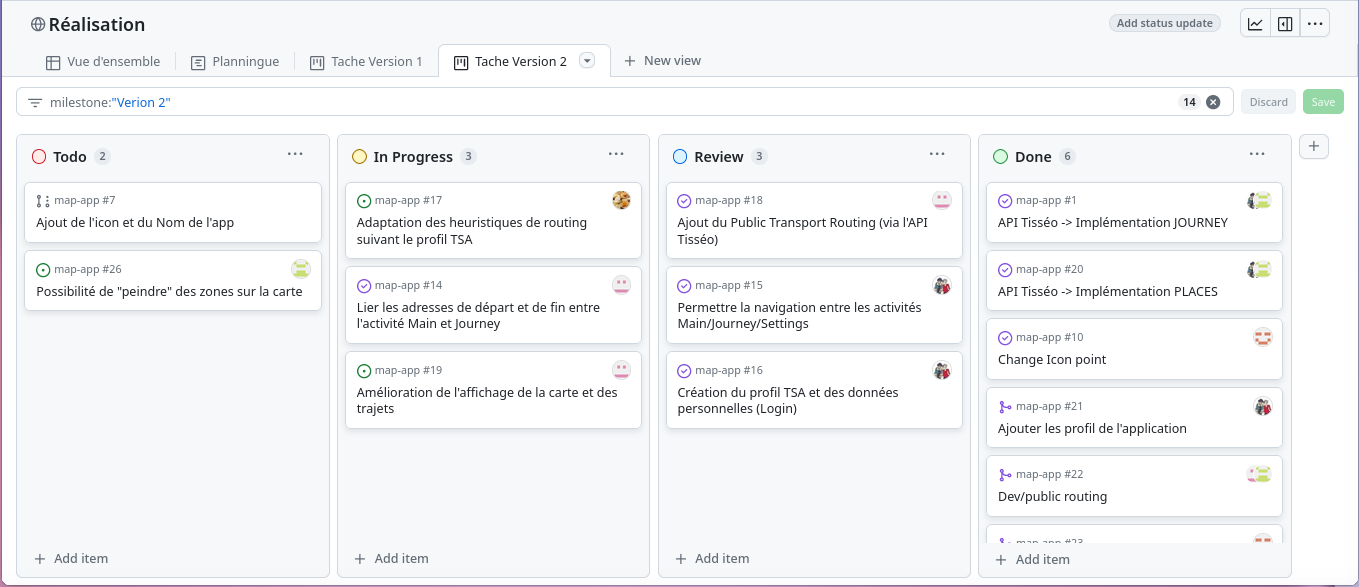
\includegraphics[width=0.8\textwidth]{img/GitHubKanban}
    \caption{GitHub Project Kanban view}
    \label{fig:GitHubKanban}
\end{figure}

We can also divide the different sprints via milestones.
This allows you to set goals with a deadline.


\newpage

Continuous integration tools like GitHub Action allow you to verify the code with each push,
but also having to be able to download an artifact.
This artifact allows us to do tests outside the development environment.
This is a great asset for code quality and development speed.


\begin{figure}[h]
    \centering
    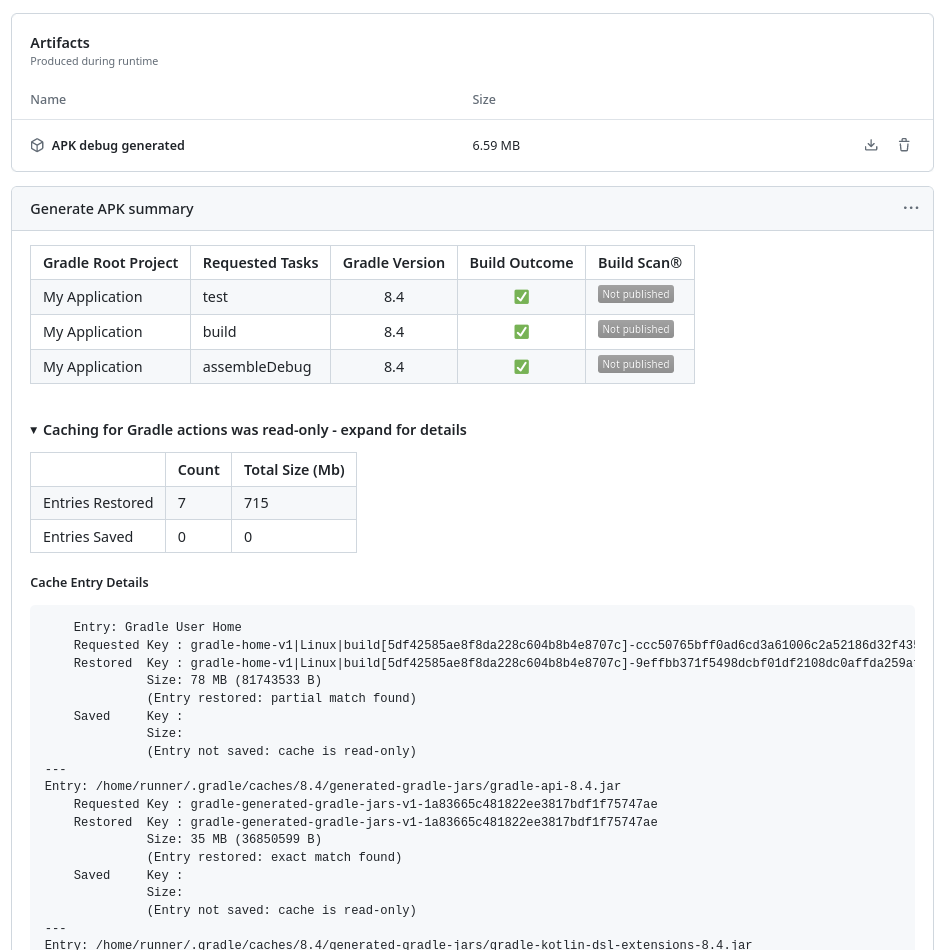
\includegraphics[width=0.4\textwidth]{img/GitHubAction}
    \caption{Workflow example with GitHub Action, with the downloadable artifact}
    \label{fig:GitHubAction}
\end{figure}


Even though GitHub Project is not as powerful as tools like Jira,
the centralization of project management accompanied by its extreme flexibility and modularity make it a perfect tool
for a modern agile method.
